\begin{titlepage}%
\begin{center}%
% Magic macro to change page borders
\newenvironment{changemargin}{%
\begin{list}{}{%
% A5 (210x148.5mm) - 1cm on all sides
\setlength{\leftmargin}{-1in+1cm}%
\setlength{\rightmargin}{-1in+1cm}%
\setlength{\textwidth}{128mm}%
\setlength{\textheight}{190mm}%
}%
\item[]}{\end{list}}%
% Then to use it
%\begin{changemargin}
%don't forget to
%\end{changemargin}
%
% More magic to adjust top margin and page length
\advance\voffset by -15.4mm % Reduce top margin from 1in to 1cm (25.4-10mm)
\advance\vsize by 115.4mm % Advance page height. The extra 100mm is to avoid a phamtom page break.
% Start graphic
\begin{changemargin}%
\vspace*{\fill}%
\noindent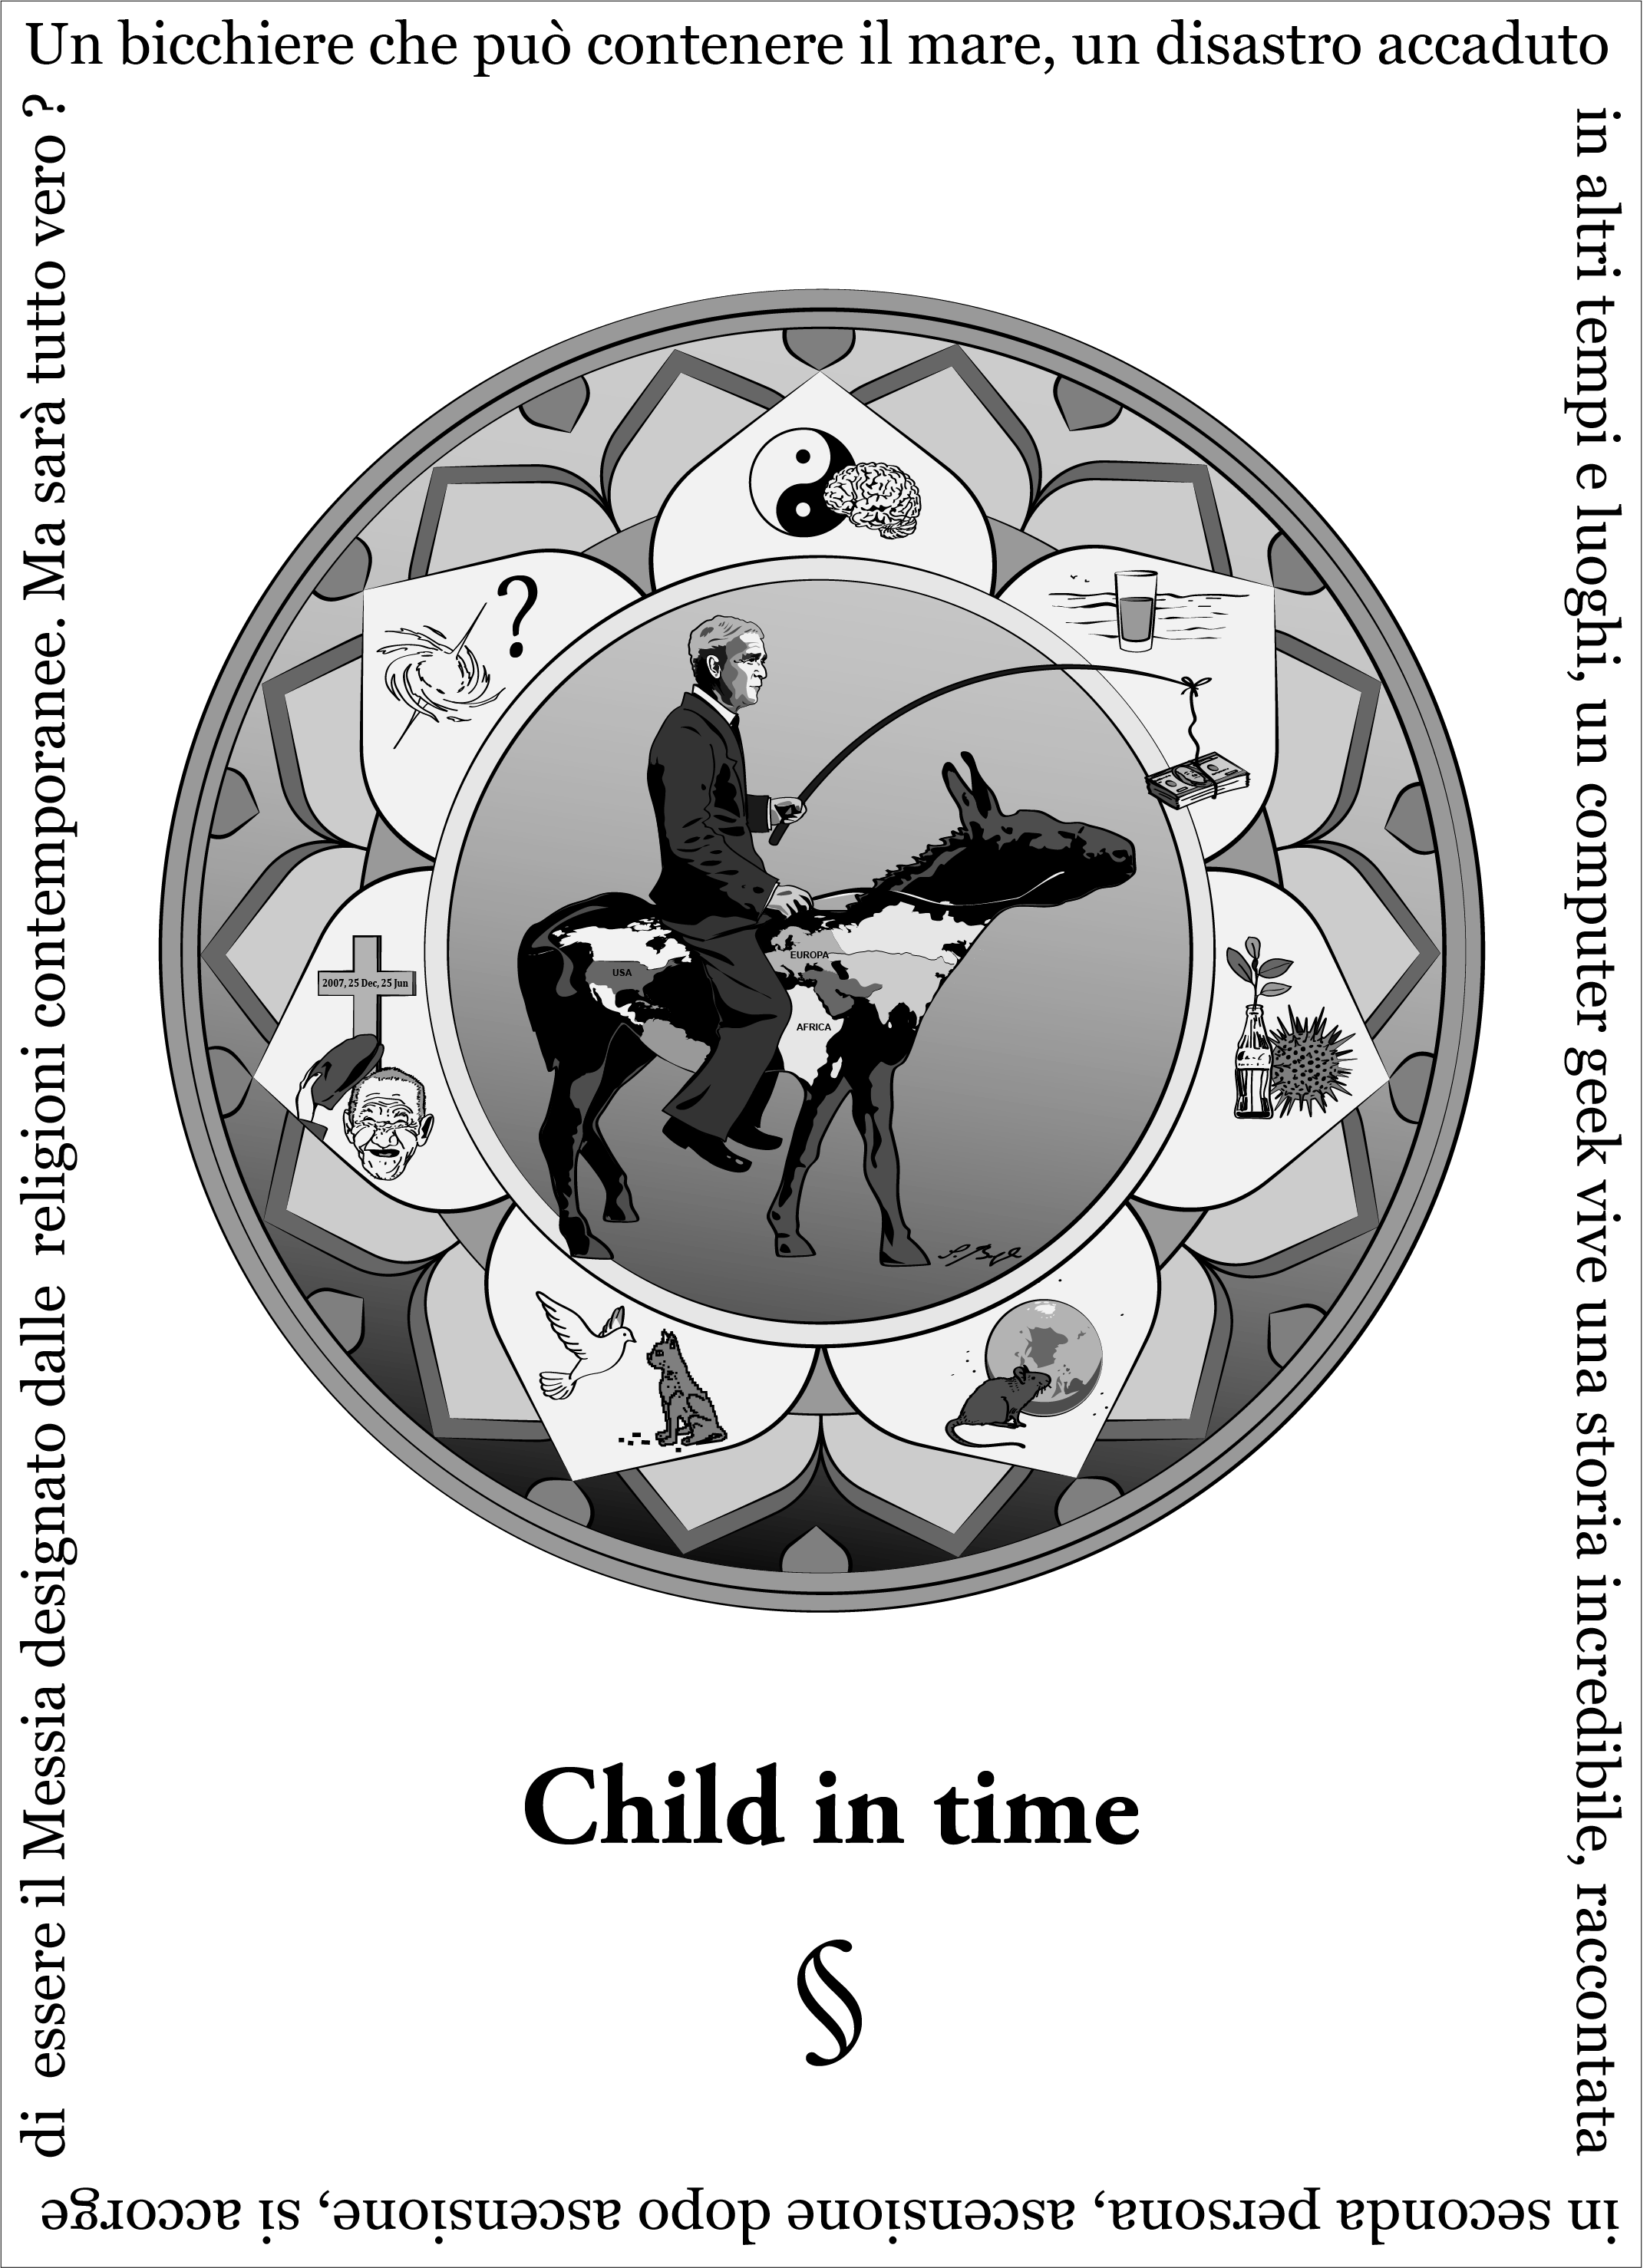
\includegraphics[width=\textwidth]{copertina-ital.png}%
\vspace*{\fill}%
\end{changemargin}%
% End graphic

\thispagestyle{empty}	% Don't print a page number on cover page

\par\vfill\break % Break the page with different margins

\advance\vsize by -115.4mm % Return old margins and page height
\advance\voffset by 15.4mm % Return old margins and page height

%\vspace*{\fill}%
\textsc{\Huge Child In Time}\\[0.5cm]
\thispagestyle{empty}	% Don't print a page number on page 2

% Title

% Author and supervisor
\begin{minipage}{0.4\textwidth}
\begin{flushleft} \large
\emph{Author:}\\
Sergio Sorrenti\\
\end{flushleft}
\end{minipage}
\begin{minipage}{0.4\textwidth}
\begin{flushright} 

{\large \today}
\end{flushright}
\end{minipage}

\vspace*{\fill}%

% Bottom of the page

\end{center}

\end{titlepage}
